\chapter{Definizione del Datawarehouse}

L'obiettivo del data warehouse in oggetto è quello di fornire dati relativi
all'utilizzo di veicoli elettrici noleggiati dalla compagnia Helbiz, nel corso
della giornata, al variare delle condizioni meteo e in presenza o assenza di uno
sciopero.
L'architettura scelta è quella a tre livelli, che vede un primo livello costituito
dalle tre sorgenti operative Helbiz, Torinometeo e Scioperi, un secondo livello
costituito consistente nell'ODS ed un terzo livello costituito dai data mart.

\section{Descrizione del dominio}
Il dominio nel quale si colloca questo progetto è quello dei monopattini elettrici noleggiati in
modalità \emph{scooter sharing}, in particolare quelli offerti dalla compagnia Helbiz sul territorio italiano.
Nella fattispecie verrà analizzato il contesto della regione Piemonte che, con Torino, ha avviato una importante
partnership con Helbiz.

Risulta quindi interessante capire quali siano gli utilizzi dei cittadini durante le diverse avversità metereologiche
anche durante le manifestazioni di astensione dal lavoro, come ad esempio gli scioperi dei mezzi pubblici.


\section{Scenario}
Lo scenario vede la nascita di un dipartimento interno di Helbiz con il compito di raccogliere dati sugli
utilizzi dei monopattini (con possibilità di estensione ad altri mezzi) in rapporto al meteo e alla presenza
o meno di scioperi nazionali, regionali o provinciali.

I dati raccolti servono principalmente ad Helbiz per diverse motivazioni:
\begin{itemize}
	\item{\textbf{Strategia} -- capire internamente in quali situazioni conviene mettere a disposizione più o meno veicoli in maniera tale da ottimizzare i costi di gestione e manutenzione.
	Questo \emph{modus operandi} consente all' azienda di poter giocare d'anticipo ed essere preparata a gestire un carico maggiore di richiesta di veicoli.}
	\item{\textbf{Promozione} -- una volta previste le necessità dell'immediato futuro, è possibile migliorare il servizio offerto ai clienti anche da un punto di vista di comunicazione,
	facendo sapere alle persone che Helbiz ha già predisposto dei piani d'emergenza nel caso di sciopero}
	\item{\textbf{Marketing} -- portare al tavolo dei Comuni non ancora serviti dal servizio dati alla mano che possano aiutare l'azienda a far capire quanto sia efficace il servizio proposto}
\end{itemize}

Al fine di arrivare a questo risultato bisogna avviare una serie di interviste che produrranno una analisi sia funzionale che tecnica;
da qui si potranno finalmente definire i requisiti  del Datawarehouse in oggetto.

\begin{table}[H]
\centering
\resizebox{\textwidth}{!}{%
\begin{tabular}{|l|l|}
\hline
\rowcolor[HTML]{3166FF} 
{\color[HTML]{FFFFFF} \textbf{Ruolo}}                                                            & {\color[HTML]{FFFFFF} \textbf{Domande}}                                                                                                                \\ \hline
                                                                                                 & Di quali tipologie di analisi vuole disporre ed a che livello di dettaglio?                                                                            \\ \cline{2-2} 
                                                                                                 & Quali sono gli obiettivi del suo dipartimento?                                                                                                         \\ \cline{2-2} 
                                                                                                 & Come misura il successo del suo dipartimento?                                                                                                          \\ \cline{2-2} 
\multirow{-4}{*}{Manager}                                                                        & Su quale intervallo temporale vuole condurre analisi?                                                                                                  \\ \hline
Cittadino                                                                                        & \begin{tabular}[c]{@{}l@{}}Pensa che possa essere utile avere informazioni sulle zone coperte da Helbiz durante\\ gli scioperi dei mezzi?\end{tabular} \\ \hline
                                                                                                 & Con quale frequenza vuole disporre delle informazioni?                                                                                                 \\ \cline{2-2} 
                                                                                                 & \begin{tabular}[c]{@{}l@{}}Quali aspetti fanno aumentare (o diminuire) drasticamente l'utilizzo dei veicoli da parte\\ dei cittadini?\end{tabular}     \\ \cline{2-2} 
\multirow{-3}{*}{Direttore della Logistica}                                                      & Qual'è la media di percorrenza di un veicolo per ogni usufruente?                                                                                      \\ \hline
                                                                                                 & Dove sono memorizzati i dati di interesse?                                                                                                             \\ \cline{2-2} 
                                                                                                 & \begin{tabular}[c]{@{}l@{}}Disponete di un team competente per la gestione ed\\ il mantenimento nel tempo del data warehouse?\end{tabular}             \\ \cline{2-2} 
\multirow{-3}{*}{\begin{tabular}[c]{@{}l@{}}Responsabile dei\\ Sistemi Informativi\end{tabular}} & Quali informazioni sono disponibili e qual’è la loro qualità?                                                                                          \\ \hline
\end{tabular}%
}
\end{table}

Logicamente questo scenario introduce una serie di complicazioni che non saranno trattate
in questo documento, ma permette di avere delle linee guida che consentono di definire
elementi fondamentali per l'analisi dei requisiti, ovvero il glossario dei requisiti e il carico di
lavoro.

\section{Glossario dei requisiti}
\begin{table}[H]
\centering
\resizebox{\textwidth}{!}{%
\begin{tabular}{|l|l|l|l|}
\hline
\rowcolor[HTML]{3166FF} 
{\color[HTML]{FFFFFF} \textbf{Fatto}} & {\color[HTML]{FFFFFF} \textbf{Possibili dimensioni}} & {\color[HTML]{FFFFFF} \textbf{Possibili misure}} & {\color[HTML]{FFFFFF} \textbf{Storicità}} \\ \hline
                                      & Condizioni atmosferiche                              &                                                  &                                           \\ \cline{2-2}
                                      & Presenza di uno sciopero                             &                                                  &                                           \\ \cline{2-2}
                                      & Data inizio periodo                                  & \multirow{-3}{*}{Numero di utilizzi}             &                                           \\ \cline{2-3}
                                      & Data fine periodo                                    &                                                  &                                           \\ \cline{2-2}
                                      & Comune                                               &                                                  &                                           \\ \cline{2-2}
\multirow{-6}{*}{Utilizzo veicolo}               & Tipo di veicolo                                      & \multirow{-3}{*}{Distanza percorsa}              & \multirow{-6}{*}{1 anno}                  \\ \hline
\end{tabular}%
}
\end{table}



\section{Carico di lavoro}
\begin{table}[h]
\centering
\begin{tabular}{|l|l|}
\hline
\rowcolor[HTML]{3166FF} 
{\color[HTML]{FFFFFF} \textbf{Fatto}} & {\color[HTML]{FFFFFF} \textbf{Interrogazione}}                                  \\ \hline
                                      & Visualizzazione utilizzi/distanze settimanali                     \\ \cline{2-2} 
                                      & Utilizzo per livelli di pioggia mese per mese                              \\ \cline{2-2} 
                                      & Confronto degli utilizzi durante uno sciopero per fascia oraria                      \\ \cline{2-2}  
                                      & Delta utilizzi al variare delle temperature a dipendere della presenza di scioperi \\ \cline{2-2} 
                                      & Numero di utilizzi durante uno sciopero nelle ore di punta         \\ \cline{2-2} 
\multirow{-7}{*}{Utilizzo veicolo}    & Numero di utilizzi durante diverse fasce orarie      \\ \hline
\end{tabular}
\end{table}
\section{Progettazione concettuale}
La progettazione concettuale comporta l’utilizzo dei requisiti identificati precedentemente 
per realizzare uno schema concettuale per il data mart. A tale scopo viene utilizzato il
Dimensional Fact Model (DFM), un modello concettuale creato appositamente per supportare
la progettazione di data mart. 
In figura~\ref{fig:dfm} è mostrato il DFM che modella il fatto relativio
all'\textbf{utilizzo di un veicolo}.

\begin{figure}[H]                                                                                                                                                            
\centering                                                                                                                                                                   
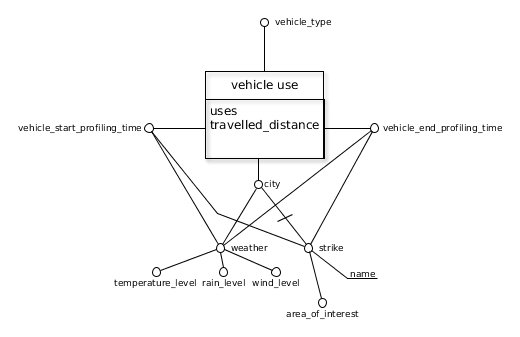
\includegraphics[width=\textwidth]{diagrams/dfm}                                                                                                                                   
\caption{DFM Vehicle use}                                                                                                                                            
\label{fig:dfm}                                                                                                                                                           
\end{figure}

Osservando il DFM si nota che gli attributi \textit{uses} e \textit{travelled\_distance}
sono le misure scelte per il fatto in questione. Entrambi gli attributi sono di tipo numerico e
rappresentano rispettivamente il numero di utilizzi e la distanza percorsa da un determinato
veicolo.
Un'istanza del fatto è identificata dalla seguenti dimensioni:
\begin{itemize}
\item \textit{start\_profiling} e \textit{end\_profiling:} dimensioni di tipo data relative
rispettivamente all'istante di inizio e di fine di una finestra di profilazione; come è possibile
notare essi condividono la gerarchia che parte dall'attributo date e comprende tutti gli 
attributi discendenti quali \textit{day}, \textit{weekday}, \textit{month}, \textit{year},
\textit{minute} e \textit{hour};
\item \textit{vehicle\_type:} dimensione di tipo stirnga che permette la selezione tra diversi
tipi di veicoli all'interno di una finestra di profilazione;
\item \textit{city:} dimensione di tipo stringa caratterizzata dall'attributo descritto di tipo
stringa \textit{name}.
\end{itemize}
Si evidenziano inolte i seguenti attributi dimensionali appartenenti alla gerarchia della
dimensione \textit{city}:
\begin{itemize}
\item \textit{weather:} attributo relativo alla rilevazione delle condizioni atmosferiche
in un determinato intervallo di tempo per una data città; esso dispone degli attributi
dimensionali \textit{weather\_start} e \textit{weather\_end} i quali condividono la gerarchia
con l'attributo \textit{date} e corrispondono a data di inizio e di fine di una rilevazione;
gli attributi descrittivi \textit{rain\_level}, \textit{temperature\_level} e
\textit{wind\_level} con i quali ogni rilevazione atmosferica è in relazione uno a uno,
permettono di descrivere con valori discreti le condizioni metereologiche in un determinato
intervallo di tempo;
\item \textit{strike:} partendo dal presupposto che non ogni città debba essere oggetto di
almeno uno sciopero, si modella tale attirbuto come opzionale per la dimensione \textit{city};
tale attributo dispone inoltre degli attributi \textit{strike\_start} e \textit{strike\_end},
che condividono la gerarchia con \textit{date}, relativi rispettivamente a 
ora di inizio e ora di fine di uno sciopero; vi sono poi gli attirbuti descrittivi \textit{name} e 
\textit{area\_of\_interest}, relativi a nome e settore interessato allo sciopero.
\end{itemize}

\section{Progettazione Logica}
In questa Sezione viene descritto il processo di trasformazione del DFM, descritto al paragrafo precedente, in modello logico. 
Innanzitutto va specificato che è stata applicata la tecnica ROLAP (Relational On-Line Analytical Processing) che prevede l’utilizzo di un
modello relazionale per la rappresentazione dei dati multidimensionali.

\begin{figure}[H]                                                                                                                                                            
\centering                                                                                                                                                                   
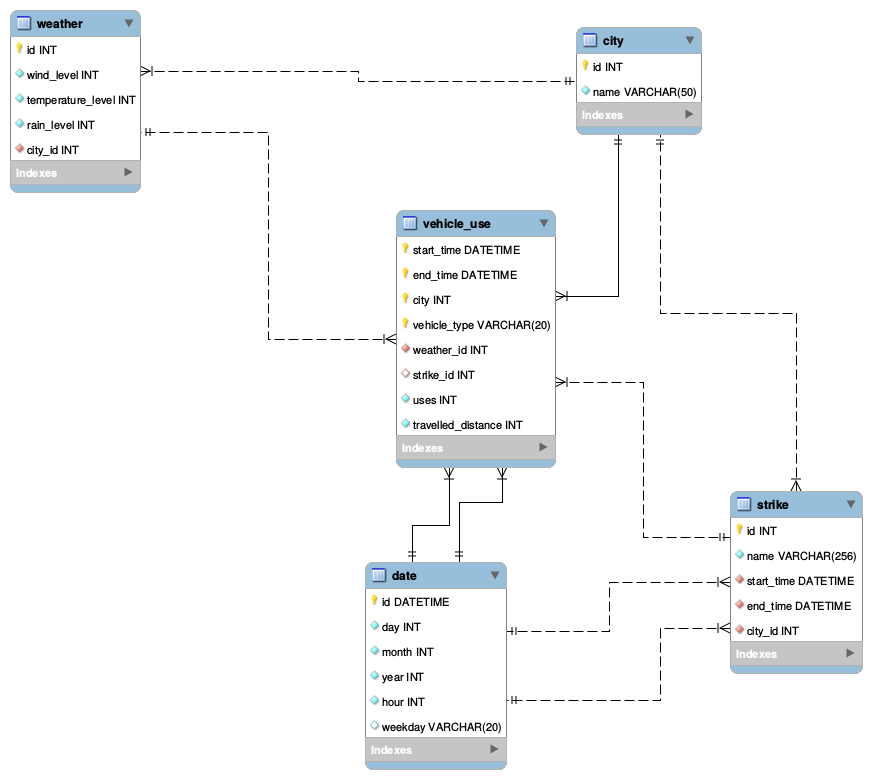
\includegraphics[width=\textwidth]{diagrams/logic}                                                                                                                                   
\caption{DFM Vehicle use}                                                                                                                                            
\label{fig:logic}                                                                                                                                                           
\end{figure}
